%% SECTION HEADER ///////////////////////////////////////////////////////////////////////////////////
\section{The numerical simulation of the \ac{gw} in the \ac{hsc} under various parameters}
\label{sec:parameters}

%% SECTION CONTENT ////////////////////////////////////////////////////////////////////////////////////
In addition to the referenced
\subsection{The \ac{pzt} parameters}
Computer simulations were conducted to determine the impact of \acp{pzt} placement relative to the core cell.
Seven transducer positions were considered, according to the schematic in Fig.~\ref{fig:pzt_place}(\textbf{b}).
The actuator and sensor position relative to the cell is identical to maintain the same wave propagation distance for each case.

From Fig.~\ref{fig:pzt_place}(\textbf{a}), it can be noticed that the highest amplitude signal is obtained for the case with the \acp{pzt} placed in the middle of the cell.
The lowest amplitudes were obtained for the cases where the transducer midpoint lay on the core wall.
It is due to the higher stiffness underneath the \ac{pzt}, leading to less displacements.
The transducers are permanently fixed to the structure and do not change their position during the monitoring period.
Nonetheless, the \acp{pzt} placement is worth considering to optimise the signals obtained.
\begin{figure}
	\begin{center}
		\includegraphics[width=0.95\textwidth]{Chapter_8/pzt_place}
	\end{center}
	\caption{The \acf{gw} propagation in the \acf{hsc} \textbf{(a)}, sensor responses for \textbf{(b)} different \acf{pzt} placement in relation to the core cell.}
	\label{fig:pzt_place}
\end{figure}

Changes in amplitude under the influence of different values of the piezoelectric charge constant and dielectric permittivity are presented in Fig.~\ref{fig:pzt_d} and ~\ref{fig:pzt_eps}, respectively.
Both parameters have a significant effect on the signal amplitude, and their values not only change with temperature but also degrade over time \cite{barzegar2001aging, deangelis2006p2o}.

\begin{figure}
	\begin{center}
		\includegraphics[width=0.95\textwidth]{Chapter_8/pzt_d}
	\end{center}
	\caption{The signal envelopes for the different piezoelectric charge constant.}
	\label{fig:pzt_d}
\end{figure}

\begin{figure}
	\begin{center}
		\includegraphics[width=0.95\textwidth]{Chapter_8/pzt_eps}
	\end{center}
	\caption{The signal envelopes for the different dielectric permittivity.}
	\label{fig:pzt_eps}
\end{figure}

\subsection{The \ac{cfrp} skin and the adhesive layer parameters}

The effect of the skin properties on wave propagation in the \ac{hsc} was analysed for different carbon fibre volume fraction in the composite.
This parameter affects the mode velocity due to the change in effective modulus of elasticity and density of the plate.
A small change in modulus velocity leads to significant signal differences within the interference of wave reflections as it can be observe in Fig.~\ref{fig:skin_volume}.
It affects the \ac{madif} determination since the full-length signal is taken into account.

\begin{figure}
	\begin{center}
		\includegraphics[width=0.95\textwidth]{Chapter_8/skin_volume}
	\end{center}
		\caption{Sensor responses in the \acf{hsc} for various fibre volume fraction in the range 45-50\%.}
	\label{fig:skin_volume}
\end{figure}

The effect of the adhesive layer thickness is presented in Fig.~\ref{fig:adhesive_thickness}.
The greater the adhesive thickness, the slower both modes propagate.
There is also a noticeable decrease in the \ac{a0} amplitude, while the \ac{s0} amplitude barely changes.
It is because the \ac{a0} displacements are mainly out-of-plane, so more energy of the wave leakages into the adhesive, and it is attenuated in low-stiffness material.

\begin{figure}
	\begin{center}
		\includegraphics[width=0.95\textwidth]{Chapter_8/adhesive_thickness}
	\end{center}
	\caption{Sensor responses in the \acf{hsc} for various adhesive thickness in the range 200-500 \(\mu\)m.}
	\label{fig:adhesive_thickness}
\end{figure}

\subsection{The core parameters}
In the study of the core geometry impact on wave propagation in \ac{hsc}, four parameters were considered:
\begin{itemize}
	\item core height \(g=[10.5,\,12.5,\,14.5,\,16.5,\,18.5]\) \unit{\mm};
	\item core width \(l_1=[5.0,\,6.0,\,7.0,\,8.0,\,9.0]\) \unit{\mm};
	\item wall thickness \(w_c=[100,\,150,\,200,\,250,\,300]\) \unit{\micro\m};
	\item core rotation angle regarding to wave propagation [\ang{0}, \ang{15}, \ang{30}, \ang{45}, \ang{60}, \ang{75}, \ang{90}].
\end{itemize}

From the signal envelopes shown in Fig.~\ref{fig:core_height}, \ref{fig:core_size}, \ref{fig:core_thickness} and \ref{fig:core_rotation} it can be seen that the analysed parameters mainly affect mode \ac{a0}. 
In contrast, for the \ac{s0}, only the amplitude changes, except for the reduction in velocity by the increase in wall thickness.

It should be mentioned that all parameters are invariable during the use of the structure and are independent of changing environmental conditions.
Therefore, the core heights and wall thicknesses are set with the dimensions tolerance received from the supplier.
The cell can easily be deformed before bonding to the skin due to the low in-plane stiffness of the core.
Thus for better accuracy, the cell width can be assumed as an average measurement value taken after joining the core with the skin.
The angle of rotation can also be corrected after the components bonding.
\begin{figure}
	\begin{center}
		\includegraphics[width=0.95\textwidth]{Chapter_8/core_height}
	\end{center}
	\caption{Sensor responses in the \acf{hsc} for the various core height in the range 10.5-18.5 \unit{\mm}.}
	\label{fig:core_height}
\end{figure}

\begin{figure}
	\begin{center}
		\includegraphics[width=0.95\textwidth]{Chapter_8/core_size}
	\end{center}
	\caption{Sensor responses in the \acf{hsc} for the various cell width in the range 5.0-9.0 \unit{\mm}.}
	\label{fig:core_size}
\end{figure}

\begin{figure}
	\begin{center}
		\includegraphics[width=0.95\textwidth]{Chapter_8/core_thickness}
	\end{center}
	\caption{Sensor responses in the \acf{hsc} for the various the wall thickness in the range 100-300 \unit{\micro\m}.}
	\label{fig:core_thickness}
\end{figure}

\begin{figure}
	\begin{center}
		\includegraphics[width=0.95\textwidth]{Chapter_8/core_rotation}
	\end{center}
	\caption{Sensor responses in the \acf{hsc} for the various core orientation.}
	\label{fig:core_rotation}
\end{figure}

\subsection{The \ac{madif} for the double-skin \ac{hsc}}

Finally, computer simulations were conducted to determine the \ac{madif} for a structure with a core between two skins.
The single-skin \ac{fcgm} from the previous analyses was supplemented with a \ac{cfrp} plate and an adhesive layer.
Two transducers were attached to the top skin as before.
Due to the impossibility of enlarging the damage in a closed-form structure, no experimental measurements were carried out.
Three damage cases were considered in the simulations: (i) interface removed from the upper side, (ii) interface removed from the bottom side and (iii) core cells removed.

Fig.~\ref{fig:rmsd_2skins} presents the \ac{rmsd}-based \ac{madif} for a double-skin panel with the functions obtained for a single skin one for comparison.
Substantial differences between the different damage models for a double skin can be observed.
For the single slab, the damage model had little significance.
In addition, the index slope is also even, mainly for the removed interface damage model, so that the damage size can be unambiguously assigned.
For the \ac{cc}-based \ac{madif}, the double-skin results are more similar to the single-plate case, as seen in Fig.~\ref{fig:cc_2skins}, especially for the top-side damage.
\begin{figure}
	\begin{center}
		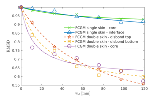
\includegraphics[width=0.95\textwidth]{Chapter_8/rmsd_2skins}
	\end{center}
	\caption{Comparison of the \acf{rmsd}-based \acf{madif} for single-skin and double-skin panel.}
	\label{fig:rmsd_2skins}
\end{figure}
\begin{figure}
	\begin{center}
		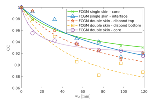
\includegraphics[width=0.95\textwidth]{Chapter_8/cc_2skins}
	\end{center}
	\caption{Comparison of the \acf{cc}-based \acf{madif} for single-skin and double-skin panel.}
	\label{fig:cc_2skins}
\end{figure}